This section describes the 3D visualisation functionality of the \into tool chain.
%
This capability is encapsulated into a Unity-based FMU that is configured and loaded into co-simulations in the usual manner.
%
Unity is a professional game engine.
%
It can be downloaded from the Unity website \cite{UnityWebsite}. 

\subsubsection{Importing the Unity Package into Unity}
To create a 3D animation FMU using Unity, first create a new project or open an existing Unity project. A Unity package was made by CLP that can be imported into Unity to expand Unity with FMU export options. This Unity package can be downloaded via the Download Manager in the INTO-CPS application or by contacting CLP.
%
First, drag-and-drop this package into the \textit{Assets} folder in Unity (in the \textit{Project} tab). See \autoref{figure:20-sim_import_unity_package} on how to import the package from the explorer into Unity. A pop-up will open, like the one shown in \autoref{figure:20-sim_import_unity_package_dialog}. Press the \textit{Import} button, as shown in \autoref{figure:20-sim_import_unity_package_dialog}.
%
\begin{figure}[ht]
	\centerline{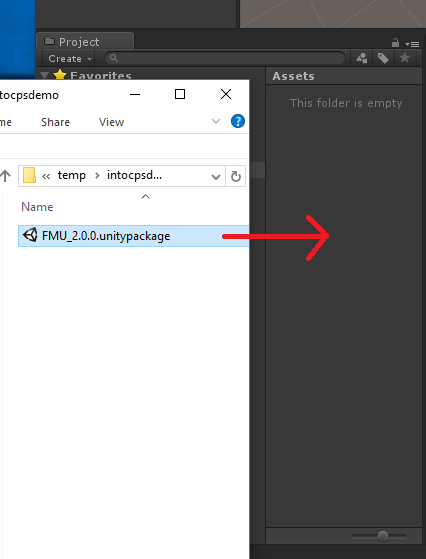
\includegraphics[width=0.6\textwidth]{figures/20sim_Unity1.png}}
	\caption{Importing the Unity package into Unity.}
	\label{figure:20-sim_import_unity_package}
\end{figure}
%
\begin{figure}[ht]
	\centerline{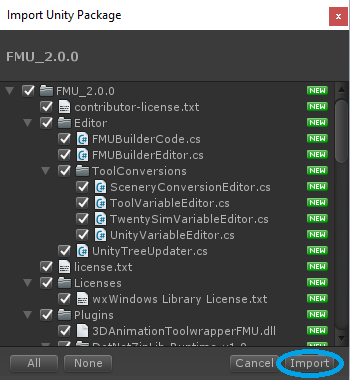
\includegraphics[width=0.4\textwidth]{figures/20sim_Unity2.png}}
	\caption{Summary of what will be imported into the Unity project.}
	\label{figure:20-sim_import_unity_package_dialog}
\end{figure}
%
Since the package contains scripts that will modify the Unity editor, it is necessary to restart the Unity project after importing the package. 
%
%
%
\subsubsection{Importing the FMUBuilder \textit{gameobject}}
After restarting Unity, go to the \textit{Hierarchy} tab. Right click within the blank part of the hierarchy (\emph{i.\@e.\@} do not select any objects in the hierarchy) and select \textit{FMU \textrightarrow FMUBuilder} (see \autoref{figure:20-sim_unity_create_fmubuilder}). This will create a new object in the hierarchy named FMUBuilder. When selecting this FMUBuilder object in the hierarchy, a few options will be shown in the \textit{Inspector} (see \autoref{figure:20-sim_unity_components_fmubuilder}). There are three components visible: \textit{Transform}, \textit{FMU Builder (Script)} and \textit{Scenery Conversion (Script)}. The latter two are unique to the INTO-CPS Unity FMU package. \textit{FMU Builder (Script)} is the component that will eventually build the 3D animation FMU, which will be covered later in this section. The other component, \textit{Scenery Conversion (Script)}, is used to convert existing 20-sim sceneries into Unity sceneries. This will also be covered later in this section.

\begin{figure}[ht]
	\centerline{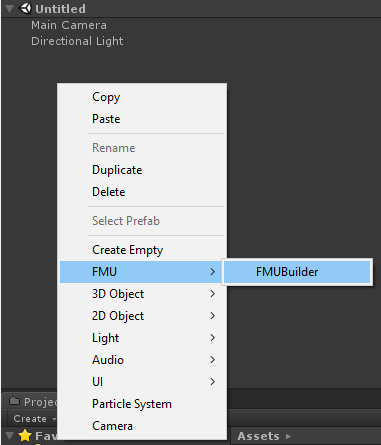
\includegraphics[width=0.5\textwidth]{figures/20sim_Unity3.png}}
	\caption{Creating the FMUBuilder \textit{gameobject} in the hierarchy tab.}
	\label{figure:20-sim_unity_create_fmubuilder}
\end{figure}

\begin{figure}[ht]
	\centerline{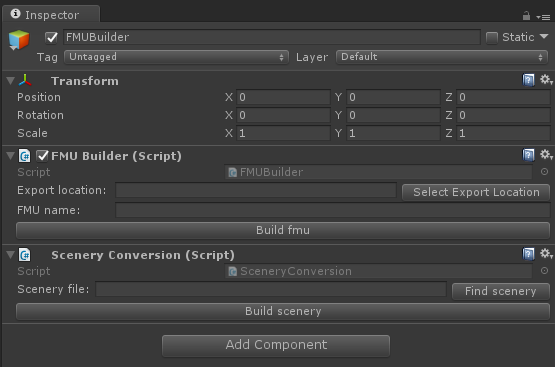
\includegraphics[width=0.7\textwidth]{figures/20sim_Unity4.png}}
	\caption{Components of the FMUBuilder in the \emph{Inspector} tab in Unity.}
	\label{figure:20-sim_unity_components_fmubuilder}
\end{figure}

\subsubsection{Assigning FMU Variables to Unity \textit{gameobject}s}
To be able to connect variables from a co-simulation to an object in Unity, a \textit{gameobject} is needed. For example, as shown in \autoref{figure:20-sim_unity_create_fmubuilder}, a cube object can be created by right-clicking in the hierarchy tab in a blank space of the hierarchy, but now selecting \textit{3D Object \textrightarrow Cube}.
%
When the newly created object is selected in the hierarchy, all components currently attached to this cube can be seen in the \textit{Inspector} tab.
%
At the bottom of this tab there is a button named \textit{Add Component}. Press this button, go to \textit{FMU variables} and choose between \textit{20-sim coordinates} or \textit{Unity coordinates}.
%
The first one means that the axes are part of a right-handed frame, that the Z-axis is pointing up, and that the order of rotation for Euler angles is X-Y-Z.
%
The latter is the Unity convention, in which the frame is left-handed, the Y-axis is pointing up, and the rotation for Euler angles is Z-X-Y.
%
See \autoref{figure:20-sim_unity_add_variable} on how to do this.
%
If there is doubt about which of the two types of variables should be chosen, choose the 20-sim option, as this is the reference frame used in most modeling tools like 20-sim.
%
Once one is selected, two additional scripts become available in the \textit{Inspector} tab. These are \textit{GUID (Script)} and either \textit{Twenty Sim Variable (Script)} or \textit{Unity Variable (Script)}. The \textit{GUID} script should not be touched. The \textit{Variable} script, however, is the script that will describe the interface variables of the to-be-generated FMU. Choose an FMU variable name and an axis, and press the \textit{Add Axis} button. Multiple axes can be defined for one \textit{gameobject}. \autoref{figure:20-sim_unity_modify_variable} shows the axes dropdown menu and the \textit{Twenty Sim Variable (Script)} and \textit{GUID (Script)} components. 

\begin{figure}[ht]
	\centerline{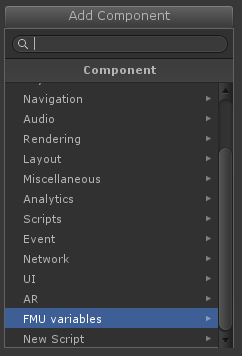
\includegraphics[width=0.4\textwidth]{figures/20sim_Unity5.png}}
	\caption{Adding new FMU variables to the Unity scene.}
	\label{figure:20-sim_unity_add_variable}
\end{figure}

\begin{figure}[ht]
	\centerline{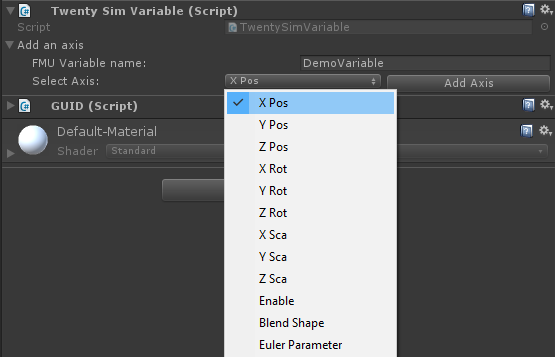
\includegraphics[width=0.7\textwidth]{figures/20sim_Unity6.png}}
	\caption{Adding the variable named "DemoVariable" for the x-position axis to the newly generated cube object.}
	\label{figure:20-sim_unity_modify_variable}
\end{figure}

\subsubsection{Converting a 20-sim Scenery into a Unity Scenery}
If a 20-sim scenery already exists, then it is possible to import it into Unity. If there is a 3D animation window in the 20-sim model, then double click the plot to open the \textit{3D Properties} window. Then go to \textit{File \textrightarrow Save Scene} (see \autoref{figure:20-sim_unity_export_scene}). If 20-sim asks to save the whole scenery, select \textit{Yes}. Remember where the scenery file is located and go back to Unity. Go to the hierarchy tab, select \textit{FMUBuilder} and enter under the \textit{Scene Conversion (Script)} the location of the scenery file, by pressing \textit{Find scenery}. Afterwards, press the \textit{Build scenery} button and the 20-sim scene will be loaded underneath the \textit{FMUBuilder} object in the hierarchy (this can be drag-dropped to other places in the hierarchy if needed), see \autoref{figure:20-sim_unity_import_scene} for the hierarchy that is created. Note that the Cube seen in \autoref{figure:20-sim_unity_export_scene} in the hierarchy is now created in Unity as well. Furthermore, the \textit{Default Lights and Cameras} frame is converted into Unity, which is a default set of lights and cameras in every 20-sim 3D scene. 
%
\begin{figure}[ht]
	\centerline{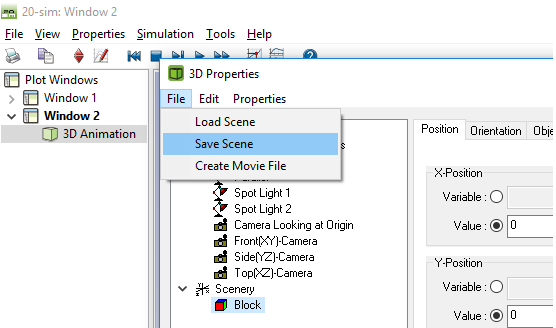
\includegraphics[width=0.7\textwidth]{figures/20sim_Unity7.png}}
	\caption{Exporting a 20-sim 3D scenery from a 3D animation plot.}
	\label{figure:20-sim_unity_export_scene}
\end{figure}
%
\begin{figure}[ht]
	\centerline{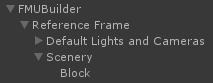
\includegraphics[width=0.3\textwidth]{figures/20sim_Unity8.png}}
	\caption{Importing a 20-sim scenery file into Unity.}
	\label{figure:20-sim_unity_import_scene}
\end{figure}
%\clearpage
%
\subsubsection{Exporting an FMU} \label{sec:simulators:20sim:fmuexport}
The final step in the process of creating a 3D animation FMU in Unity is the build process itself. The variables that were added by manually assigning FMU variables to \textit{gameobject}s and by importing 20-sim scenery files will now be used to generate the FMU itself. Every variable name (either the ones manually entered, or automatically generated by the import 20-sim scenery option) will be the input variables of this FMU. Select the \textit{FMUBuilder} in the hierarchy and go to the \textit{Inspector} tab. Under \textit{FMU Builder (Script)} select the export location and the name of the to-be-exported FMU, then press \textit{Build FMU}. Once the build process is done, the FMU will be present in the export location selected, with the given name. Note that for larger Unity scenes this can take a while to build.
